\documentclass[10pt,aspectratio=169]{beamer}

\usetheme{Madrid}
\usecolortheme{dolphin}
\setbeamertemplate{navigation symbols}{}
\setbeamertemplate{footline}[frame number]
\setbeamertemplate{bibliography item}{}

\usepackage{booktabs}
\usepackage{amsmath}
\usepackage{xcolor}
\usepackage{tikz}
\usetikzlibrary{arrows.meta, positioning}
\usepackage{graphicx}
\usepackage{colortbl}
\usepackage{array}
\usepackage[round,authoryear]{natbib}

\definecolor{accentblue}{RGB}{0,80,160}
\definecolor{accentred}{RGB}{180,30,30}
\definecolor{lightblue}{RGB}{220,235,255}
\definecolor{wingreen}{RGB}{210,245,210}
\definecolor{loserose}{RGB}{255,220,220}

\title[Functional Load Forecasting]{Functional Forecasting of Turkish Electricity Load Curves}
\author{Zeynep Bozoklu \\[0.3em] \small Advisor: Prof. Nazarii Salish}
\institute{Department of Economics, Universidad Carlos III Madrid}
\date{\today}

\begin{document}

% ============================================================
% SLIDE 1: TITLE
% ============================================================
\begin{frame}
  \titlepage
\end{frame}

% ============================================================
% SLIDE 2: THE OBJECT: A CURVE, NOT 24 NUMBERS
% ============================================================
\begin{frame}{The object: a curve, not 24 numbers}
  \begin{columns}
    \begin{column}{0.62\textwidth}
      \includegraphics[width=\linewidth]{../output/figs/fda_mean_actual_forecast_all.png}
    \end{column}
    \begin{column}{0.35\textwidth}
      \Large $Y_d(h),\quad h=0,\ldots,23$
      \vspace{0.6em}

      \normalsize
      \begin{itemize}
        \item One coherent daily trajectory
        \item Ramp, plateau, and evening peak are
              \emph{features of the whole curve},
              not isolated hours
        \item Official (dashed) sits below actual
              at every hour
        \item \textbf{Goal:} forecast tomorrow's
              full profile $Y_{d+1}(\cdot)$
      \end{itemize}
    \end{column}
  \end{columns}
\end{frame}

% ============================================================
% SLIDE 3: THE PROBLEM AND THE STAKES
% ============================================================
\begin{frame}{The problem and the stakes}
  \begin{columns}
    \begin{column}{0.45\textwidth}
      \small
      \begin{tabular}{lrr}
        \toprule
        Year & Official bias & Our bias \\
             & (MWh/hr) & (MWh/hr) \\
        \midrule
        2023 & $+344$ & $+176$ \\
        2024 & $+585$ & $+34$  \\
        2025 & $+472$ & $+98$  \\
        \midrule
        \textbf{Avg} & $\mathbf{+467}$ & $\mathbf{+103}$ \\
        \bottomrule
      \end{tabular}\\[0.4em]
      \small Positive = actual $>$ forecast (underprediction).\\[0.5em]
      \textbf{Users affected:}
      \begin{itemize}\small
        \item TEİAŞ --- unit commitment, reserves
        \item Generators --- day-ahead bids
        \item Large consumers --- imbalance penalties
      \end{itemize}
    \end{column}
    \begin{column}{0.52\textwidth}
      \textbf{Why does the official underpredict?}\\[0.3em]
      \small The mechanism is \emph{left open}.
      Candidate explanations (tentative speculation only):
      \begin{itemize}
        \item \textbf{Model update lags:} structural demand growth
              outpaces recalibration.
              The 2024 row ($+585$ MWh) is consistent.
        \item \textbf{Growing demand:} persistent trend the
              official model may be slow to incorporate.
      \end{itemize}
    \end{column}
  \end{columns}
\end{frame}

% ============================================================
% SLIDE 4: RESEARCH QUESTION
% ============================================================
\begin{frame}{Research question}
  \textbf{Main RQ:}
  \textit{Can a functional model of the daily load curve
  statistically outperform the official TEİAŞ day-ahead forecast?}\\[0.2em]

  \vspace{0.8em}
  \begin{enumerate}
    \item \textbf{Sub-Q1 (Representation).}
          Do B-spline smoothing and FPCA represent Turkey's daily
          load curves with negligible information loss?
          How many components suffice?

    \vspace{0.4em}
    \item \textbf{Sub-Q2 (Linearity).}
          Is the linear score equation adequate, or does a nonlinear
          model \emph{outside} the FPCA setting suggest unexploited
          structure in the data?
  \end{enumerate}

  \vspace{0.7em}
  \footnotesize
  \textit{Literature positioning is provisional, pending the
  systematic review. No prior FDA study of Turkish electricity
  demand has been located.
  FDA framework: \citep{ramsay_2005, kokoszka_2017, hyndman_2007}.}
\end{frame}

% ============================================================
% SLIDE 5: METHOD: THE PIPELINE
% ============================================================
\begin{frame}{Method: the pipeline}
  \vspace{-0.4em}
  \begin{center}
  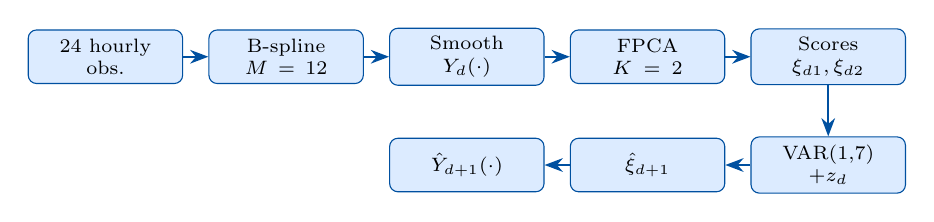
\begin{tikzpicture}[
    node distance=0.38cm and 0.32cm,
    box/.style={rectangle, rounded corners=3pt, draw=accentblue, fill=lightblue,
                text width=1.75cm, align=center, font=\scriptsize,
                minimum height=0.68cm, inner sep=3pt},
    arr/.style={-Stealth, thick, accentblue}
  ]
    \node[box] (raw)    {24 hourly\\obs.};
    \node[box, right=of raw]    (spline) {B-spline\\$M=12$};
    \node[box, right=of spline] (curve)  {Smooth\\$Y_d(\cdot)$};
    \node[box, right=of curve]  (fpca)   {FPCA\\$K=2$};
    \node[box, right=of fpca]   (scores) {Scores\\$\xi_{d1},\xi_{d2}$};
    \node[box, below=0.65cm of scores] (var) {VAR(1,7)\\$+z_d$};
    \node[box, left=of var]  (hatsc) {$\hat\xi_{d+1}$};
    \node[box, left=of hatsc](recon) {$\hat Y_{d+1}(\cdot)$};
    \draw[arr] (raw)--(spline); \draw[arr] (spline)--(curve);
    \draw[arr] (curve)--(fpca); \draw[arr] (fpca)--(scores);
    \draw[arr] (scores)--(var); \draw[arr] (var)--(hatsc);
    \draw[arr] (hatsc)--(recon);
  \end{tikzpicture}
  \end{center}
  \vspace{0.1em}
  \begin{columns}
    \begin{column}{0.52\textwidth}
      \small
      \vspace{-0.3em}
      \[
        Y_d(h)=\mu(h)+\textstyle\sum_k \xi_{dk}\varphi_k(h)+\varepsilon_d(h)
      \]
      \vspace{-0.7em}
      \[
        \xi_d = a + A_1\xi_{d-1} + A_7\xi_{d-7} + Bz_d + u_d
      \]
      \vspace{-0.7em}
      \[
        \hat{Y}_d(h) = \hat\mu(h) + \hat\varphi_1(h)\hat\xi_{d1} + \hat\varphi_2(h)\hat\xi_{d2}
      \]
      \vspace{-0.3em}
      \scriptsize OLS, equation-by-equation. All $z_d$ predetermined.\\[0.2em]
      \scriptsize FPCA: \citep{ramsay_2005, kokoszka_2017};
      functional forecasting: \citep{hyndman_2007}
    \end{column}
    \begin{column}{0.45\textwidth}
      \small
      \begin{tabular}{lp{0.56\textwidth}}
        \toprule
        Block & Key content \\
        \midrule
        Calendar      & Weekend, annual sine/cosine \\
        \textbf{Holiday} & Public holidays, bridge days \\
        Load shape    & Mean, peak, range, rolling avg.\ \\
        \textbf{Deriv.} & Morning/evening ramp ($DY_{d-1}$) \\
        \bottomrule
      \end{tabular}
      \vspace{0.3em}
      \scriptsize \textbf{Rolling-origin / expanding window:}
      all $z_d$ strictly predetermined $\Rightarrow$ \textbf{no leakage}.
      Underpins all results.
    \end{column}
  \end{columns}
\end{frame}

% ============================================================
% SLIDE 6: FPCA: TWO SCORES CAPTURE THE CURVE (Sub-Q1)
% ============================================================
\begin{frame}{FPCA: two scores capture the curve (Sub-Q1)}
  \begin{columns}
    \begin{column}{0.60\textwidth}
      \includegraphics[width=\linewidth]{../output/figs/eigenfunction_shape_comparison.png}
    \end{column}
    \begin{column}{0.37\textwidth}
      \small
      \begin{tabular}{rrr}
        \toprule
        FPC & Var. & Cumul. \\
        \midrule
        1 & 93.4\% & 93.4\% \\
        2 &  3.9\% & 97.3\% \\
        3 &  1.1\% & 98.4\% \\
        4 &  1.0\% & 99.4\% \\
        \bottomrule
      \end{tabular}

      \vspace{0.5em}
      \textbf{FPC 1 (level):} nearly flat
      $\Rightarrow$ uniform lift/drop.

      \vspace{0.3em}
      \textbf{FPC 2 (shape):} positive overnight/evening,
      negative daytime\\
      $\Rightarrow$ peak-vs-plateau contrast.

      \vspace{0.5em}
      $K=4$ adds $<1\%$ variance; results unchanged.

      \vspace{0.3em}
      \textit{Static FPCA is a compromise between
      simplicity and dimension reduction, not a
      claim of optimality.}
    \end{column}
  \end{columns}
\end{frame}

% ============================================================
% SLIDE 7: MAIN RESULTS: BUILDING THE MODEL (Main RQ)
% ============================================================
\begin{frame}{Main results: building the model (Main RQ)}
  \begin{center}
  \small
  \begin{tabular}{p{0.38\textwidth}rrrrc}
    \toprule
    Model & MAE & MAPE & vs.\ off. & DM stat & \\
    \midrule
    Seasonal na\"{i}ve $Y_{d-7}$ & 1912 & 5.13\% & $-57.6\%$ & $+35.2$ & \\
    \textbf{Official (TEİAŞ)}    & \textbf{1214} & \textbf{3.15\%}
                                  & ref. & --- & \\
    \midrule
    FPCA VAR(1,7) only           & 1443 & 3.76\% & $-18.9\%$ & $+22.9$ & \\
    $+$ calendar / ramp          & 1238 & 3.26\% & $-2.1\%$  & $+2.6$  & \\
    \rowcolor{wingreen}
    $+$ holiday / load-shape     & 1001 & 2.63\% & $+17.5\%$ & $-24.9$ & *** \\
    \rowcolor{wingreen}
    $+$ derivative features      & \textbf{980} & \textbf{2.56\%}
                                  & $+19.2\%$ & $-27.4$ & *** \\
    \midrule
    \rowcolor{wingreen}
    $+$ residual correction      & \textbf{653} & \textbf{1.70\%}
                                  & $+46.2\%$ & $-71.2$ & *** \\
    \bottomrule
  \end{tabular}
  \end{center}
  \vspace{0.1em}
  \footnotesize
  Negative DM stat = better than official; ***$\,p<0.001$.\ \
  \textbf{DM significant at 18 of 24 hours} (hour-by-hour; pooled $p$ is secondary).\ \
  MAE in MWh/hour.\ \ Evaluation: 1,096 days / 26,304 hourly errors, 2023--2025.\ \
  DM test: \citet{dm_1995}; HLN small-sample correction: \citet{hln_1997}.
\end{frame}

% ============================================================
% SLIDE 8: WHERE IT LOSES, AND THE RESIDUAL STEP
% ============================================================
\begin{frame}{Where it loses, and the residual step}
  \begin{columns}
    \begin{column}{0.48\textwidth}
      \includegraphics[width=\linewidth]{../output/figs/fpca_VAR_1_7_gain_vs_official_by_hour.png}
      \vspace{0.15em}
      \scriptsize Positive = model beats official (MAE).\\
      \textcolor{accentred}{\textbf{Hours 6--9:}} ramp timing is
      temperature-driven; at hr 8, MAPE loss $\approx$24\%.\\
      Errors are autocorrelated: Ljung--Box up to 7,227 at h6.
    \end{column}
    \begin{column}{0.49\textwidth}
      \includegraphics[width=\linewidth]{../output/figs/acf_base_vs_correction.png}
      \vspace{0.05em}
      \small Correction:
      \[
        \hat{Y}_d^{\text{res}} = \hat{Y}_d^{\text{base}} + \lambda_d\hat{r}_d
      \]
      $\lambda_d,\hat{r}_d$ from strictly pre-$d$ data (rolling CV)
      $\Rightarrow$ no leakage.\\[0.4em]
      \textbf{Result:} $+46.2\%$ MAE, DM stat $-71.2$.\\
      Wins at \textbf{all 24/24 hours}.\\[0.3em]
      \scriptsize Residual correction approach: \citep{xie_2016}
    \end{column}
  \end{columns}
\end{frame}

% ============================================================
% SLIDE 9: LINEARITY: IS THE LINEAR MODEL ADEQUATE? (Sub-Q2)
% ============================================================
\begin{frame}{Linearity: is the linear model adequate? (Sub-Q2)}
  \begin{columns}
    \begin{column}{0.55\textwidth}
      \includegraphics[width=\linewidth]{../output/figs/direct_RF_mae_by_hour_load_only.png}
    \end{column}
    \begin{column}{0.42\textwidth}
      Main model: \textbf{OLS on FPCA scores}

      \vspace{0.4em}
      \textbf{Probe:} direct RF predicting hourly load
      directly, bypassing FPCA entirely.
      Same features $+$ lagged hourly values.

      \vspace{0.5em}
      \scriptsize
      \begin{tabular}{lrrc}
        \toprule
        Model & MAE & vs.\ off. & \\
        \midrule
        Official (2025) & 1052 & ref. & \\
        \rowcolor{wingreen}
        FPCA-OLS (2025) & 910  & $+13.5\%$ & *** \\
        \rowcolor{wingreen}
        Direct RF (2025) & \textbf{718} & $+31.8\%$ & *** \\
        \bottomrule
      \end{tabular}

      \vspace{0.5em}
      \footnotesize
      \textbf{Reading (open):} linear is adequate \emph{within}
      the FPCA-score structure; the single-year RF gain hints
      at structure the FPCA compression discards.
      
    \end{column}
  \end{columns}
\end{frame}

% ============================================================
% SLIDE 10: CONCLUSION
% ============================================================
\begin{frame}{Discussion and Conclusion}
  \begin{itemize}
    \item \textbf{Expand the nonlinear probe to the full horizon.}\\[0.2em]
          {\small Direct RF's single-year gain ($+31.8\%$ on 2025 alone) is
          the clearest empirical lead. The natural next step is to extend
          the evaluation to the full 2023--2025 rolling-origin window
          and test whether the structural gain holds out of sample.}

    \vspace{0.5em}
    \item \textbf{Develop the economic story of the underprediction.}\\[0.2em]
          {\small The $\approx$467 MWh/hour systematic bias is observed but
          unexplained. The thesis should characterise which curve
          segments drive it and connect this to the institutional
          context of the Turkish electricity market.}

    \vspace{0.5em}
    \item \textbf{Complete the systematic literature review.}\\[0.2em]
          {\small FDA applied to electricity demand is an active area.
          Positioning the contribution requires a structured survey.}
  \end{itemize}

  \vspace{0.4em}
  \footnotesize The core empirical results --- FPCA representation,
  VAR pipeline, DM-confirmed accuracy, residual correction ---
  are complete and validated. No new data collection required.
\end{frame}

% ============================================================
% SLIDE 11: REFERENCES
% ============================================================
\begin{frame}{References}
  \footnotesize
  \begin{thebibliography}{99}
    \bibitem[Ramsay and Silverman(2005)]{ramsay_2005}
    Ramsay, J.O.\ \& Silverman, B.W.\ (2005).
    \textit{Functional Data Analysis}, 2nd ed.\ Springer.

    \bibitem[Kokoszka and Reimherr(2017)]{kokoszka_2017}
    Kokoszka, P.\ \& Reimherr, M.\ (2017).
    \textit{Introduction to Functional Data Analysis}. CRC Press.

    \bibitem[Hyndman and Ullah(2007)]{hyndman_2007}
    Hyndman, R.J.\ \& Ullah, M.S.\ (2007).
    Robust forecasting of mortality and fertility rates.
    \textit{Computational Statistics \& Data Analysis}, 51(10), 4942--4956.

    \bibitem[Diebold and Mariano(1995)]{dm_1995}
    Diebold, F.X.\ \& Mariano, R.S.\ (1995).
    Comparing predictive accuracy.
    \textit{J.\ Business \& Economic Statistics}, 13(3), 253--263.

    \bibitem[Harvey et al.(1997)]{hln_1997}
    Harvey, D., Leybourne, S.\ \& Newbold, P.\ (1997).
    Testing the equality of prediction mean squared errors.
    \textit{Intl.\ J.\ Forecasting}, 13(2), 281--291.

    \bibitem[Xie and Hong(2016)]{xie_2016}
    Xie, J.\ \& Hong, T.\ (2016).
    GEFCom2014 probabilistic electric load forecasting.
    \textit{Intl.\ J.\ Forecasting}, 32(3), 1012--1016.
  \end{thebibliography}
\end{frame}

\end{document}
